% GMC-Link — ACM Multimedia Asia 2026 Regular Paper
% Double-blind submission: sigconf + review + anonymous.
% Build: latexmk -pdf main.tex   (acmart.cls from system TeX Live)
\documentclass[sigconf,anonymous,nonacm]{acmart}

\usepackage{multirow}              % per-host recipe table
\usepackage{microtype}             % kills sub-3pt overfull, polishes justification
\usepackage{tikz}                  % Fig 1 pipeline + Fig 2 ego-motion schematic (self-contained, no asset)
\usetikzlibrary{arrows.meta,positioning,fit,backgrounds}
\captionsetup{textfont={normalfont}}  % bold label, normal description (lead-in phrases bolded per caption)
\settopmatter{printacmref=false}   % no ACM ref block in review draft
\setcopyright{none}
\acmConference[MM Asia '26]{ACM International Conference on Multimedia in Asia}{December 2026}{Location TBD}
\acmYear{2026}
\settopmatter{printfolios=false}    % pure paper copy without reviewer page numbers
\renewcommand\footnotetextcopyrightpermission[1]{} % remove ACM conference/copyright footer
\emergencystretch=1em

\begin{document}

\title{Recovering Motion-Referring Expressions in Moving-Camera Videos via Global Motion Compensation}

\author{Anonymous Author(s)}
\affiliation{%
  \institution{Submission under double-blind review}
  \country{}
}

\begin{abstract}
Referring multi-object tracking takes a video and a natural-language expression and tracks every object the expression describes. Many expressions refer to how an object moves rather than how it looks, but common hosts read motion from raw box displacement. A moving camera corrupts that signal: a parked car sweeps across the frame and is scored as ``moving,'' while a car keeping pace with traffic can read as static and be dropped. Motion-language RMOT fuses dynamics with text yet leaves the camera in the signal; ego-motion compensation removes the camera but is used only for association. We connect the two with a decision-level plug-in: per-frame homographies compose into a cumulative transform, residual velocity is read at multiple gaps, a two-tower encoder aligns it with the expression, and the score is added to the host logit without host retraining. On iKUN, aligning motion with language lifts moving-class HOTA by $+8.83$ (native $20.25\!\to\!29.08$, $n{=}5$); most of that lift comes from giving the host any motion descriptor, while ego-compensation is the only engineered component with a significant effect and the only one that serves both directions of the disambiguation: removing it costs $-1.77$ moving ($p{=}0.006$) and $-2.07$ static-class HOTA ($p{<}10^{-4}$), the parked objects that raw velocity misreads as moving. Across three host--split settings, the recovered signal is monotone-inverse to native motion ability. In pooled HOTA the module matches iKUN's published score and improves FlexHook's V2 score outright ($+0.281$), while FlexHook V1 remains below its published number under a known reproduction gap.
\end{abstract}

\keywords{referring multi-object tracking, ego-motion compensation, motion-language alignment, plug-in module, Refer-KITTI, video grounding}

\maketitle
\thispagestyle{empty}
\pagestyle{empty}

\section{Introduction}
\label{sec:intro}

Referring multi-object tracking (RMOT) outputs trajectories for the objects described by a free-form sentence, and many such sentences describe motion rather than appearance. Queries such as ``moving cars'' or ``a vehicle turning left'' require actual object motion. However, the usual image-plane displacement mixes two sources: the object's motion and the camera's ego-motion. That mixture fails systematically under a moving camera. A stationary car can sweep across the image and be scored as ``moving'', while a genuinely moving car can keep a nearly fixed image column when its motion cancels the camera's. The signal a motion-class query depends on is exactly the signal a moving camera corrupts.

The two research lines that could fix this have not met. Motion-language RMOT, including VMRMOT~\cite{vmrmot} and its RMOT lineage~\cite{transrmot,ikun,flexhook}, aligns dynamics with text but derives those dynamics from camera-contaminated image-plane trajectories. Plain MOT has camera compensation: BoT-SORT~\cite{botsort} and UCMCTrack~\cite{ucmctrack} estimate camera motion and stabilize predictions, but the corrected geometry is consumed by association and never exposed to language. The missing capability is therefore not merely ``GMC plus text''. It is a persistent, ego-stable object-motion representation, accumulated over the temporal span of a motion expression, and explicitly aligned with language. Platform pose is in principle available from KITTI GPS/IMU or ground-plane projection, but to our knowledge no RMOT method routes it to language; a feature-based estimate keeps the module sensor-free (no GPS/IMU required) and architecture-agnostic across the two-stage hosts we target, at the price of the per-host scalar calibration of Section~\ref{sec:fusion}.

GMC-Link occupies that intersection. Per-frame homographies estimate camera motion; their cumulative transform gives an ego-stable reference for each track; multi-gap residual velocity turns that reference into a temporal motion descriptor; a contrastive aligner scores whether the descriptor matches the expression; and a calibrated decision-level correction adds only that motion evidence to the host logit. The cumulative transform is central: it makes the descriptor reflect the object rather than the camera and lets the evidence persist across the window a motion verb spans. This yields a falsifiable hypothesis. If ego-compensation matters beyond merely adding motion features, replacing residual velocity with raw velocity should cost recovery on the moving class and misread parked objects on the static class. Section~\ref{sec:exp} tests exactly that and reports the decomposition: the descriptor itself carries most of the moving-class lift, and ego-compensation is the component that makes it a disambiguator rather than a motion prior.

This work connects the mature ego-motion-compensation machinery of plain tracking with the emerging motion--language line of RMOT, and makes the following contributions.
\begin{itemize}
  \item A plug-in motion-language module that compensates ego-motion, keeps the host detector, tracker, and appearance grounding unchanged, and attaches through a calibrated decision-level correction rather than host retraining.
  \item A cross-setting characterization over iKUN (V1) and FlexHook (V1/V2) showing that gain follows a monotone-inverse ordering with native motion ability; FlexHook V1/V2 are one architecture on two splits, so they are not independent architectural confirmations.
  \item Mechanism evidence decomposing the $+8.83$ moving-class recovery: a raw-velocity descriptor already supplies $+7.06$, and ego-compensation contributes the remaining $+1.77$ on the moving class (Welch $p{=}0.006$) plus $+2.07$ on the static class ($p{<}10^{-4}$) --- the only statistically significant engineered component, and the one that restores parked objects that raw velocity misreads as moving. Decision-level fusion is the viable injection site after feature-level injection regresses.
\end{itemize}

On iKUN~\cite{ikun}, the module matches published pooled HOTA~\cite{hota} while lifting the motion class hidden by the appearance-heavy pooled metric; on FlexHook~\cite{flexhook} V2, it improves pooled HOTA outright. The gains hold at a fixed tracker and are orthogonal to detector quality: reaching the top of the leaderboard requires a stronger tracker than the public detections expose, which is out of scope for a plug-in that changes neither the detector nor the host.

\section{Related Work}
\label{sec:related}

\subsection{Referring MOT and motion-language fusion}
TransRMOT~\cite{transrmot} established RMOT on Refer-KITTI, iKUN~\cite{ikun} decoupled grounding from association through a frozen tracker, and FlexHook~\cite{flexhook} strengthened the two-stage cross-modal hook. The two-stage referring-by-tracking line continues to grow, with zero-shot MLLM captioning over frozen tracks (ReferGPT~\cite{refergpt}) and memory-efficient plug-in referring modules (MEX~\cite{mex}). Later RMOT methods improve semantic grounding~\cite{mlstrack,deeprmot,cdrmot,tellmewhat}; VMRMOT~\cite{vmrmot} even makes motion explicit with position, direction, distance-trend, and speed-trend descriptors. The common limitation is where the dynamics come from: raw image-plane boxes. Thus motion-language RMOT can be language-aware while its motion representation remains entangled with camera ego-motion. TempRMOT~\cite{temprmot} already aggregates trajectory history in recurrent memory, and we exclude such hosts on evidence rather than convenience: cascading the module onto TempRMOT regressed pooled HOTA in two independent trials ($-6.75$ under an early cascade rule, $-3.8$ to $-5.4$ across a later coefficient sweep), consistent with an external motion module adding redundant constraints to a host whose recurrent state already encodes trajectory history.

\subsection{Camera and ego-motion compensation in tracking}
Camera compensation is standard in plain MOT, where it stabilizes predictions before association. BoT-SORT~\cite{botsort} estimates an inter-frame transform from ORB matches~\cite{orb} with RANSAC~\cite{ransac}, while UCMCTrack~\cite{ucmctrack} uses a ground-plane camera-motion model. EMAP~\cite{emap} goes furthest in this direction, decoupling camera rotation and translation from object motion inside the Kalman prediction itself and improving KITTI HOTA by over $5\%$ across four trackers. All three improve association under ego-motion, but the corrected geometry is consumed immediately by frame-to-frame association. It is not composed into a persistent ego-stable trajectory, accumulated over the temporal span of a motion expression, or exposed as a language-aligned feature. The geometric core we rely on is classical --- plane-plus-parallax motion separation~\cite{iranianandan}, homography estimation~\cite{hartleyzisserman}, motion segmentation under a moving camera~\cite{bideau}, and ego-motion estimation in visual odometry~\cite{scaramuzza} --- and we claim no novelty in the separation itself; the contribution is routing its output to language.

\subsection{The unfilled intersection}
The gap is specific: motion-language RMOT is language-aware but camera-contaminated; camera-compensated MOT is ego-stable but language-unaware. GMC-Link connects them by producing persistent ego-stable motion, aligning it with the expression, and fusing it after the host score. The method therefore preserves host appearance grounding while supplying the motion evidence that the host never had.

\section{Method}
\label{sec:method}

GMC-Link sits between a two-stage RMOT host and its scoring step. The host remains responsible for detection, association, and appearance-language grounding. The GMC branch estimates background camera motion and converts host tracks into ego-stable residual object motion. The aligner asks whether that residual motion matches the referring expression, and fusion adds only a calibrated correction after the host has formed its appearance-based score. This modularity enables post-hoc attachment without replacing the detector, retraining host weights, or hiding the source of a correction. Figure~\ref{fig:architecture} gives the attachment point, and Figure~\ref{fig:pipeline} shows the four stages.

The separation is also diagnostic: failures can be assigned to host appearance grounding, ego-motion estimation, motion-language alignment, or scalar calibration instead of to an opaque fused representation.

\begin{figure*}[t]
\centering
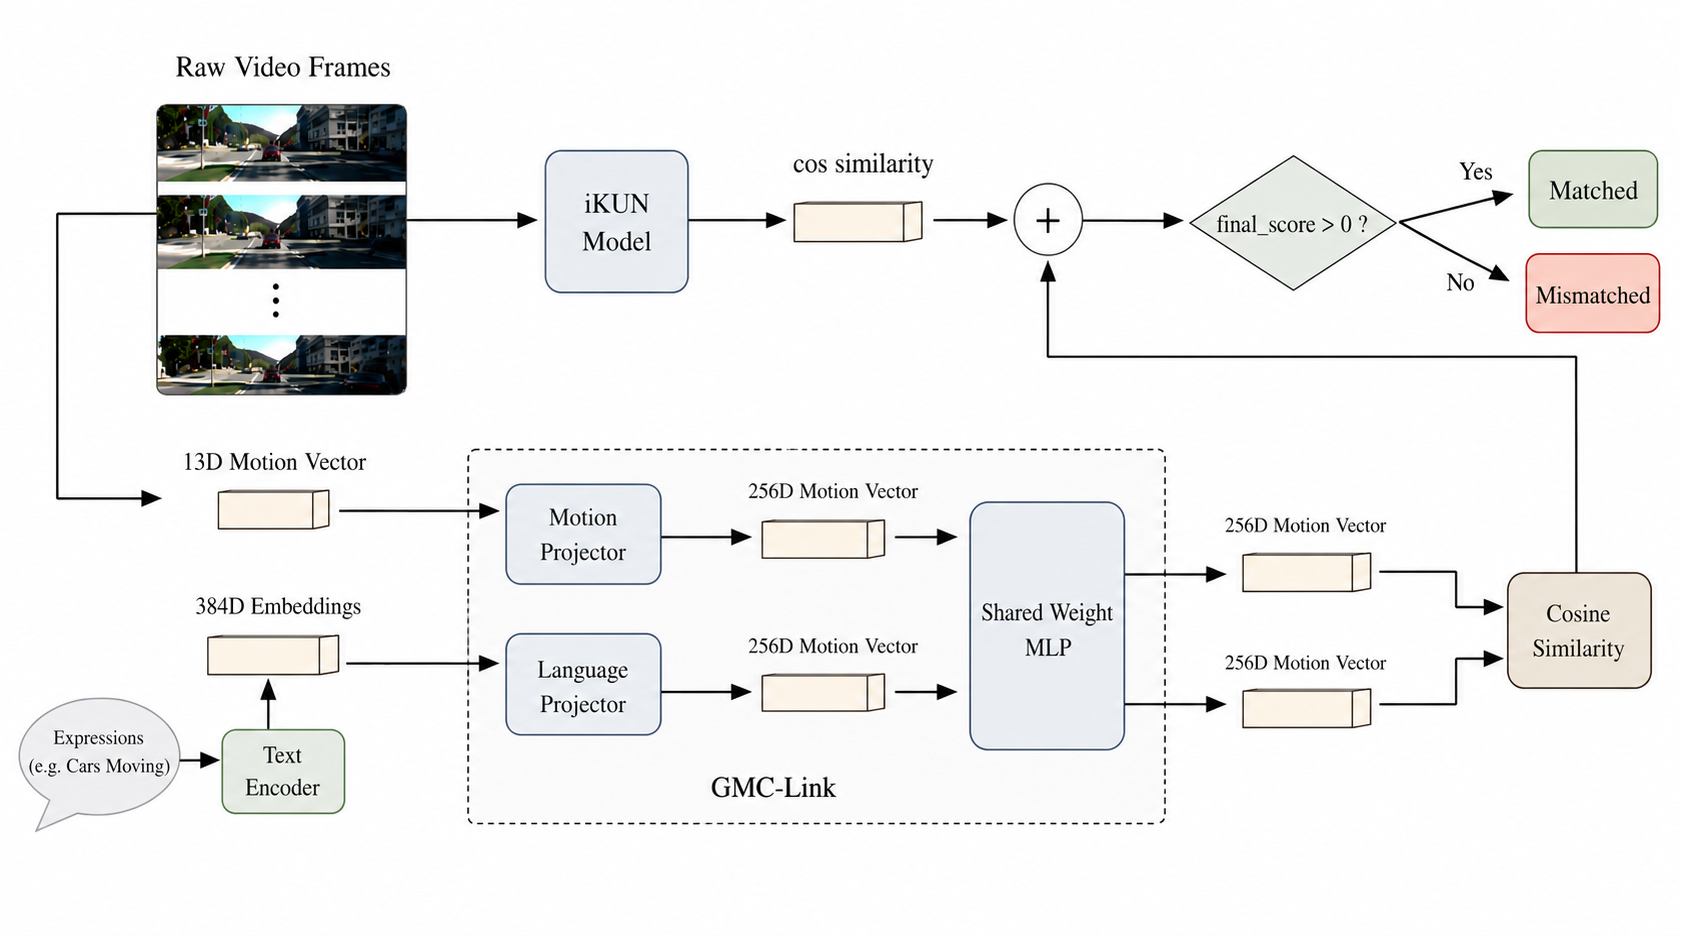
\includegraphics[width=0.82\textwidth]{figures/Architecture.png}
\caption{\textbf{GMC-Link architecture.} The host provides tracks and expression scores; GMC-Link estimates camera motion, derives residual motion, aligns it with language, and returns only a calibrated decision-layer correction.}
\label{fig:architecture}
\end{figure*}

\begin{figure}[t]
\centering
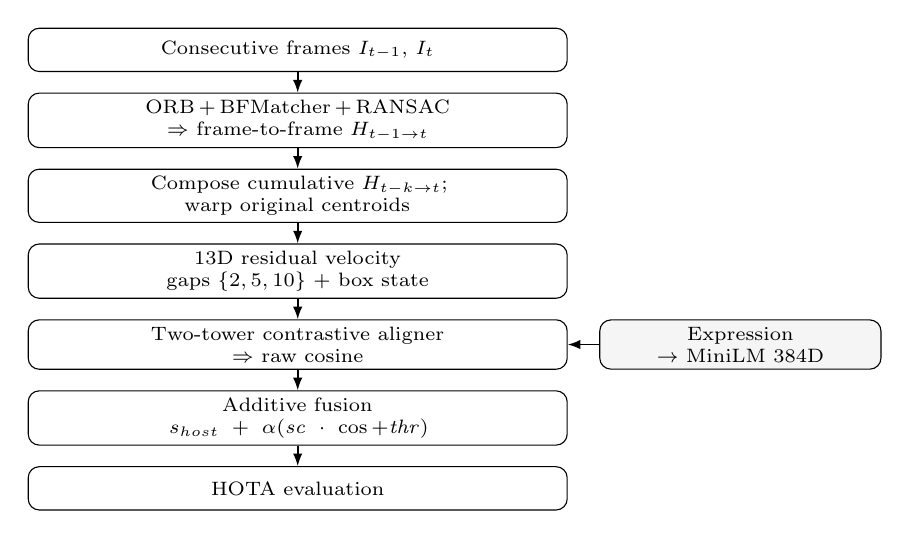
\begin{tikzpicture}[
  font=\scriptsize,
  node distance=2.6mm,
  box/.style={draw, rounded corners, align=center, inner sep=2.5pt,
              text width=0.55\linewidth, minimum height=5.5mm},
  sbox/.style={draw, rounded corners, align=center, inner sep=2.5pt, fill=black!4,
               text width=0.28\linewidth, minimum height=5.5mm},
  ar/.style={-{Latex[length=1.6mm]}, semithick}
]
\node[box] (frames) {Consecutive frames $I_{t-1},\,I_t$};
\node[box, below=of frames] (orb) {ORB\,+\,BFMatcher\,+\,RANSAC\\ $\Rightarrow$ frame-to-frame $H_{t-1\to t}$};
\node[box, below=of orb] (cum) {Compose cumulative $H_{t-k\to t}$;\\ warp original centroids};
\node[box, below=of cum] (desc) {13D residual velocity\\ gaps $\{2,5,10\}$ + box state};
\node[box, below=of desc] (align) {Two-tower contrastive aligner\\ $\Rightarrow$ raw cosine};
\node[box, below=of align] (fuse) {Additive fusion\\ $s_{\text{host}}+\alpha(\mathit{sc}\cdot\cos+\mathit{thr})$};
\node[box, below=of fuse] (hota) {HOTA evaluation};
\node[sbox, right=4mm of align] (text) {Expression\\ $\to$ MiniLM 384D};
\draw[ar] (frames)--(orb);
\draw[ar] (orb)--(cum);
\draw[ar] (cum)--(desc);
\draw[ar] (desc)--(align);
\draw[ar] (align)--(fuse);
\draw[ar] (fuse)--(hota);
\draw[ar] (text)--(align);
\end{tikzpicture}
\caption{\textbf{GMC-Link pipeline.} ORB homographies compose into a cumulative transform, produce a 13D residual-velocity descriptor, align with the expression, and correct the host logit for HOTA evaluation.}
\label{fig:pipeline}
\end{figure}

\subsection{Ego-motion compensation}
\label{sec:ego}

The first stage estimates camera motion between adjacent frames. We use ORB as a sparse feature-point sampler because global camera motion should be estimated from repeatable, matchable background evidence rather than from every image location. Dense sampling or dense optical flow supplies many more measurements, but in driving footage many of those measurements come from weak-texture road regions, object boundaries, reflections, residual parallax, and independently moving foreground objects; these ambiguous samples can introduce high-volume noise and bias a single global transform. ORB instead keeps a compact set of discriminative corners with binary descriptors, making descriptor matching and later outlier rejection more reliable and efficient. We detect ORB keypoints~\cite{orb}, match descriptors with a brute-force Hamming matcher, and keep matches passing Lowe's $0.7$ ratio test. Host boxes seed a foreground mask: without masking, correspondences on moving objects can bias the transform away from background camera motion, so keypoints inside tracked objects are suppressed and the surviving matches better represent static scene structure. RANSAC~\cite{ransac} fits $H_{t-1\to t}$ and records median inlier reprojection error as background residual. If too few reliable inliers survive, the stage falls back to identity, so a weak-texture frame degrades to ``no compensation'' rather than to a corrupted camera-motion estimate.

A single homography is exact only for planar or pure-rotation scenes, but driving footage is sufficiently planar-dominated for this approximation to be useful. In our data, ORB with RANSAC outperformed dense optical flow because explicit feature selection and outlier rejection discard noisy or non-background measurements that a dense field tends to smear into the estimate. Frame-to-frame compensation is still insufficient for language, because motion expressions span multiple frames. We therefore store the original, never-warped centroids and compose the frame-to-frame transforms into one cumulative homography,
\begin{equation}
H_{t-k\to t} = H_{t-1\to t}\, H_{t-2\to t-1} \cdots H_{t-k\to t-k+1},
\label{eq:cumulative}
\end{equation}
then apply it once to map a past centroid into the current frame. This creates a persistent ego-stable reference while avoiding the error that would accumulate from repeatedly warping already-warped coordinates.

\subsection{Multi-scale residual velocity}
\label{sec:residual}

For temporal gap $g$, raw velocity is centroid displacement and contains both object motion and camera-induced displacement. Ego velocity estimates the displacement caused by the camera alone by warping the past centroid through Eq.~\ref{eq:cumulative}. Residual velocity is their difference,
\begin{equation}
v^{\mathrm{res}}_{g} = v^{\mathrm{raw}}_{g} - v^{\mathrm{ego}}_{g},
\label{eq:residual}
\end{equation}
which approximates the motion a stationary camera would observe. Thus a parked car has near-zero residual motion even as its pixels move significantly under ego-motion. We normalise by image dimensions, $v_{\mathrm{norm}} = (v_{\mathrm{pix}}/d_{\mathrm{img}})\times 100$.

We compute residuals at gaps $\{2,5,10\}$ and concatenate them with box state into a 13D vector ordered as $(\mathit{dx}_s,\mathit{dy}_s)$, $(\mathit{dx}_m,\mathit{dy}_m)$, $(\mathit{dx}_l,\mathit{dy}_l)$, $\Delta w,\Delta h,c_x,c_y,w,h,\mathit{snr}$; the first six entries are residual $(dx,dy)$ pairs at gaps $2$, $5$, and $10$. The scales are complementary rather than redundant. Gap $2$ preserves short-term changes and jitter that long windows average away; gap $10$ accumulates slow sustained motion that can be buried in one short step; gap $5$ bridges the regimes. This matters for language because expressions may refer to instantaneous changes or sustained movement over different temporal spans. The final $\mathit{snr}$ is the mid-scale residual object speed relative to the RANSAC-inlier background noise floor. It does not create class separation itself, but represents homography reliability and reduces frame-level score variance when compensation is weak.

\subsection{Motion-language alignment}
\label{sec:align}

A two-tower encoder maps the 13D motion vector and expression into a shared space. Linear adapters (motion $13\!\to\!256$, language $384\!\to\!256$ from all-MiniLM-L6-v2~\cite{sbert}) feed a shared MLP ($256\!\to\!512\!\to\!512\!\to\!256$), layer norm, and $\ell_2$ normalisation. Training uses symmetric InfoNCE~\cite{infonce} at temperature $0.07$ with shared-expression false negatives masked. Inference uses raw cosine similarity, with no sigmoid or temporal smoothing, so fusion receives an uncalibrated alignment score. The aligner is intentionally standard: the scientific claim is not a new text encoder or contrastive loss, but that ego-compensated residual motion is the right signal to align. CLIP-text and larger 768D sentence encoders did not consistently improve the shipped raw-cosine pipeline, so MiniLM stays.

\subsection{Decision-level additive fusion}
\label{sec:fusion}

The alignment score corrects the host logit at the decision level. We inject it additively per host and per axis,
\begin{equation}
s_{\mathrm{final}} = s_{\mathrm{model}} + \alpha\,\bigl(\mathit{sc}\cdot\cos + \mathit{thr}\bigr),
\label{eq:fusion}
\end{equation}
where $\cos$ is raw motion-language cosine, $\mathit{sc}$ rescales it to the host logit range, $\mathit{thr}$ shifts the operating point, and $\alpha$ sets weight. We use decision-level fusion because feature-level motion injection into the visual encoder regressed an early pipeline by $-21.7\%$ F1; one negative trial does not establish decision-level fusion as optimal, but it motivates keeping motion evidence out of the host's appearance representation. The final design therefore preserves the host's appearance representation and injects motion only after the host has formed its score. This keeps appearance grounding intact, prevents motion features from distorting the visual representation, and leaves host evidence and motion evidence as separate auditable terms.

A keyword router selects the motion recipe when an expression contains one of $15$ fixed motion substrings (e.g.\ \emph{moving}, \emph{turning}, \emph{parked}, \emph{braking}); otherwise it selects the appearance recipe. Because motion evidence is largely uninformative for appearance-only expressions, $\mathit{sc}_{\mathrm{appear}}$ is seven to eleven times smaller than $\mathit{sc}_{\mathrm{motion}}$. The coefficients absorb host-specific logit-scale differences, so the table should be read as calibration to each host's score range rather than as a learned fusion head.

\begin{table}[t]
\centering
\caption{Locked fusion coefficients for Eq.~\ref{eq:fusion}, hand-set per host--split setting. FlexHook (V1) and (V2) are one architecture calibrated per split. Appearance scale is damped because motion is uninformative on appearance expressions.}
\label{tab:recipe}
\small
\begin{tabular}{llccc}
\toprule
Host & Axis & $\alpha$ & $\mathit{sc}$ & $\mathit{thr}$ \\
\midrule
\multirow{2}{*}{iKUN}        & motion     & 1.00 & 0.90 & $+0.17$ \\
                             & appearance & 1.00 & 0.30 & $+0.10$ \\
\midrule
\multirow{2}{*}{FlexHook (V1)} & motion     & 0.65 & 10.0 & $+3.0$  \\
                             & appearance & 1.00 & 3.50 & $+0.9$  \\
\midrule
\multirow{2}{*}{FlexHook (V2)} & motion     & 0.40 & 10.0 & $+1.3$  \\
                             & appearance & 1.00 & 3.50 & $+1.2$  \\
\bottomrule
\end{tabular}
\end{table}

Standard-deviation matching and a learned fusion network were tested but underperformed this fixed scalar calibration. This is consistent with the plug-in goal: a new host needs calibration to its score range, but not retraining of its detector, tracker, visual encoder, or language grounding pathway.

\section{Experiments}
\label{sec:exp}

\subsection{Setup}
\label{sec:setup}

We evaluate on Refer-KITTI V1~\cite{transrmot} and V2~\cite{temprmot} using TrackEval HOTA~\cite{hota}. Moving-class HOTA tests whether the module fixes the target failure; pooled HOTA checks whether that recovery survives the full benchmark. Comparing iKUN~\cite{ikun} with FlexHook~\cite{flexhook} tests whether the gain concentrates where native motion reasoning is weakest, and the raw-velocity ablation tests whether ego-compensation matters beyond adding any motion descriptor. FlexHook (V1/V2) is one architecture calibrated per split, not two independent methods. Results are mean$\pm$std over $n{=}3$ seeds for cross-setting tables and $n{=}5$ for ablations with Welch tests; a seed randomizes aligner training (initialization and batch order) only, while homography estimation and host outputs are deterministic. The aligner uses AdamW ($10^{-3}$, batch $256$, $100$ epochs); ORB uses $1500$ features and RANSAC a $5$\,px threshold. All iKUN comparisons use the paper-canonical ground-truth template aligned with the public NeuralSORT detections, and each host runs its published public detections unchanged. We report native hosts and a simple uncalibrated raw-cosine GMC control to separate adding the signal from calibrating it to the host logit scale. Code, trained aligner weights for every seed, per-sequence score caches, and the coefficient tables will be released upon publication.

Refer-KITTI has no held-out tuning split, so Table~\ref{tab:recipe}'s shipped coefficients are calibrated on the benchmark sequences and should not be claimed as universally transferable hyperparameters. Two observations bound the fitting capacity. First, the scale coefficients were calibrated independently per FlexHook split yet came out identical ($\mathit{sc}{=}10.0$ motion, $3.5$ appearance on both V1 and V2 in Table~\ref{tab:recipe}), suggesting the calibration tracks the host's logit range rather than the particular test sequences; with those shared, roughly four fitted scalars per setting remain against three to four evaluation sequences. Second, we use leave-one-sequence-out calibration to bound overfitting risk directly. iKUN LOSO moving HOTA remains $28.38 \pm 1.60$ versus $29.47 \pm 0.88$ in-sample (native $20.25$), while FlexHook LOSO pooled is $53.28 \pm 0.17$ (V1) and $42.74 \pm 0.07$ (V2), with V2 still above the published $42.526$. We therefore claim the iKUN moving-class recovery and the FlexHook V2 pooled gain, not the iKUN pooled number, as calibration-robust.

The test splits are heavily skewed toward appearance. V1 holds $158$ expressions over $1010$ frames, of which $75.3\%$ are appearance queries, $7.6\%$ are static-motion queries, and only $17.1\%$ ($27$ expressions) refer to a moving object; V2 holds $862$ expressions over $1469$ frames with a similar $74.1\,/\,11.7\,/\,14.2$ split. The motion class our module targets is therefore a roughly one-in-six minority. Pooled HOTA is computed once over the union of all trajectories, so it is dominated by detection and association counts from the appearance majority; it is not a class-weighted mean of per-class HOTA. A recovery concentrated on moving expressions can therefore register as a small pooled movement even when the per-class effect is large. The module's target failure is motion-class grounding, so moving-class HOTA is the pre-specified effect metric rather than a post-hoc selection; pooled HOTA is the field-standard whole-benchmark summary, reported for every setting with all deltas anchored to the native host.

\subsection{Main results}
\label{sec:main}

Table~\ref{tab:main} first shows that raw GMC evidence is not sufficient by itself: the uncalibrated \emph{+GMC simple} control is negative on iKUN and FlexHook V1. The signal must be calibrated to the host's score range. With the shipped calibration, iKUN~\cite{ikun} reaches $44.634 \pm 0.066$, matching rather than materially beating the published $44.564$, while FlexHook V2 gives the clean pooled improvement, $42.807 \pm 0.038$ versus $42.526$ ($+0.281$). Pooled parity on iKUN should be read as a guarantee rather than a shortfall: the moving-class recovery is purchased at no cost to the roughly $83\%$ of queries the module does not target, which is the property that makes a plug-in safe to attach. FlexHook V1 improves over \emph{+GMC simple} ($53.121 \to 53.526$) but remains below its published $53.824$: no tested configuration beats that number --- the strongest legacy variant reaches $53.716 \pm 0.068$ ($n{=}3$) --- so we treat the V1 gap as a reproduction limit of our pipeline and report the module's V1 gain against the \emph{+GMC simple} control. The scientific claim is therefore not that GMC-Link beats every pooled leaderboard number; it is that ego-compensated motion recovers motion-class errors, especially where native motion reasoning is weakest. For external context, VMRMOT~\cite{vmrmot}, the strongest motion-language host on this benchmark, reports $53.00$/$35.21$ pooled HOTA on V1/V2 with its own end-to-end detector and tracker. The FlexHook settings with our module reach $53.526$/$42.807$ on the same splits, but we attribute that ordering to host and pipeline rather than to the module and do not claim a head-to-head win; the class-level comparison our claim would require is not computable from published numbers, as VMRMOT does not report per-class moving HOTA. We therefore compare each host against its own native score.

\begin{table}[t]
\centering
\caption{Pooled HOTA on Refer-KITTI test ($n{=}3$, mean$\pm$std). $\Delta$ is against published pooled HOTA; iKUN matches, while FlexHook V2 is the clean pooled improvement.}
\label{tab:main}
\small
\setlength{\tabcolsep}{4pt}
\begin{tabular}{lcccc}
\toprule
Host & Native & +GMC simple & +GMC (ship) & $\Delta$ paper \\
\midrule
iKUN~\cite{ikun} (V1)        & 44.564 & 44.272 & $44.634 \pm 0.066$ & $+0.070$ \\
FlexHook (V1)~\cite{flexhook}  & 53.824 & 53.121 & $53.526 \pm 0.087$ & $-0.298$\textsuperscript{$\dagger$} \\
FlexHook (V2)~\cite{flexhook}  & 42.526 & 42.532 & $42.807 \pm 0.038$ & $+0.281$ \\
\bottomrule
\end{tabular}
\\[2pt]
{\footnotesize \textsuperscript{$\dagger$}FlexHook (V1) paper gap is structural (no tested configuration beats $53.824$); $\Delta$ vs \emph{+GMC simple} anchor $= +0.405$.}
\end{table}

\subsection{The motion deficit}
\label{sec:deficit}

The gain tracks native motion deficit. iKUN starts lowest and gains most ($+8.83 \pm 0.83$); FlexHook V1 and V2 start higher and gain little ($+0.91 \pm 0.79$ and $+0.43 \pm 0.17$). Across the three settings, the relation is monotone-inverse: larger native deficit receives larger correction. This supports the intended use case, a host that already grounds appearance but does not reliably distinguish ego-induced displacement from object motion. We treat the pattern as a prediction over three settings --- effectively two independent architectures, since the FlexHook pair shares weights-in-kind --- not a proportional law; confirming it as a characterization requires further hosts.

\begin{table}[t]
\centering
\caption{Motion deficit across host--split settings. Native moving-class HOTA versus the moving-class HOTA gain added by the module. The gain is monotone-inverse to native motion ability across the three settings; the FlexHook rows are one architecture calibrated per split.}
\label{tab:deficit}
\small
\begin{tabular}{lcc}
\toprule
Host & Native MOVING & GMC MOVING gain \\
\midrule
iKUN~\cite{ikun}             & 20.25 & $+8.83 \pm 0.83$ ($n{=}5$) \\
FlexHook (V1)~\cite{flexhook}  & 43.98 & $+0.91 \pm 0.79$ ($n{=}3$) \\
FlexHook (V2)~\cite{flexhook}  & 48.02 & $+0.43 \pm 0.17$ ($n{=}3$) \\
\bottomrule
\end{tabular}
\\[2pt]
{\footnotesize Moving-class denominators: $27$ of $158$ expressions (V1); $14.2\%$ of $862$ (V2).}
\end{table}

\subsection{Ablations}
\label{sec:ablation}

The ablation directly tests the Introduction hypothesis, and we report the decomposition rather than the headline alone. The full module lifts the moving class $20.25\to29.08$ ($+8.83$); the $-$ego arm, which feeds raw uncompensated velocity to the same aligner, already reaches $27.31$, so having a motion descriptor at all supplies $+7.06$ of the recovery and ego-compensation the remaining $+1.77$ (Welch $t{=}3.75$, $p{=}0.006$, $95\%$ CI $[0.67, 2.87]$, Cohen's $d{\approx}2.4$). The moving class understates what compensation buys, because raw velocity errs in both directions: on the static class, the $-$ego arm drops $43.26\to41.19$, a $-2.07$ cost ($t{=}9.81$, $p{<}10^{-4}$) concentrated exactly on the parked objects whose pixels sweep across the frame. Single-gap motion ($-0.26$ moving, $p{=}0.64$) and removing snr ($+0.67$ moving, $p{=}0.19$) stay within seed spread on both classes, so ego-compensation is the only statistically significant engineered component, and the only one the disambiguation claim rests on; its effect survives Bonferroni correction over the three component tests ($p_{\mathrm{corr}}{=}0.018$). Two caveats keep the null results honest: at $n{=}5$ they bound only large effects, so modest multiscale or snr contributions cannot be excluded, and the $-$snr arm's higher mean is itself within that spread --- snr is retained as the variance-reduction feature of Section~\ref{sec:residual}, and dropping it would be a defensible simplification rather than a loss.

\begin{table}[t]
\centering
\caption{Per-class HOTA ablation on iKUN ($n{=}5$). Ego-compensation is the only significant engineered component, and the only one that moves both classes: removing it costs $-1.77$ moving (Welch $p{=}0.006$) and $-2.07$ static ($p{<}10^{-4}$).}
\label{tab:ablation}
\small
\begin{tabular}{lcc}
\toprule
Variant & MOVING HOTA & STATIC HOTA \\
\midrule
Native host (no module)           & 20.25 & --- \\
Full module                       & \textbf{29.08 $\pm$ 0.83} & \textbf{43.26 $\pm$ 0.26} \\
\;\;$-$ego (raw velocity)         & 27.31 $\pm$ 0.66 & 41.19 $\pm$ 0.39 \\
\;\;$-$multiscale (single gap)    & 28.82 $\pm$ 0.84 & 43.42 $\pm$ 0.10 \\
\;\;$-$snr                        & 29.74 $\pm$ 0.59 & 43.35 $\pm$ 0.35 \\
\bottomrule
\end{tabular}
\\[2pt]
{\footnotesize Native static-class HOTA under the ablation readout is not archived; deltas among module arms share one convention and are directly comparable.}
\end{table}

Feature-level injection regressed an early host by $-21.7\%$ F1, supporting the decision to correct logits after appearance scoring rather than reshaping host representations.

\begin{figure}[t]
\centering
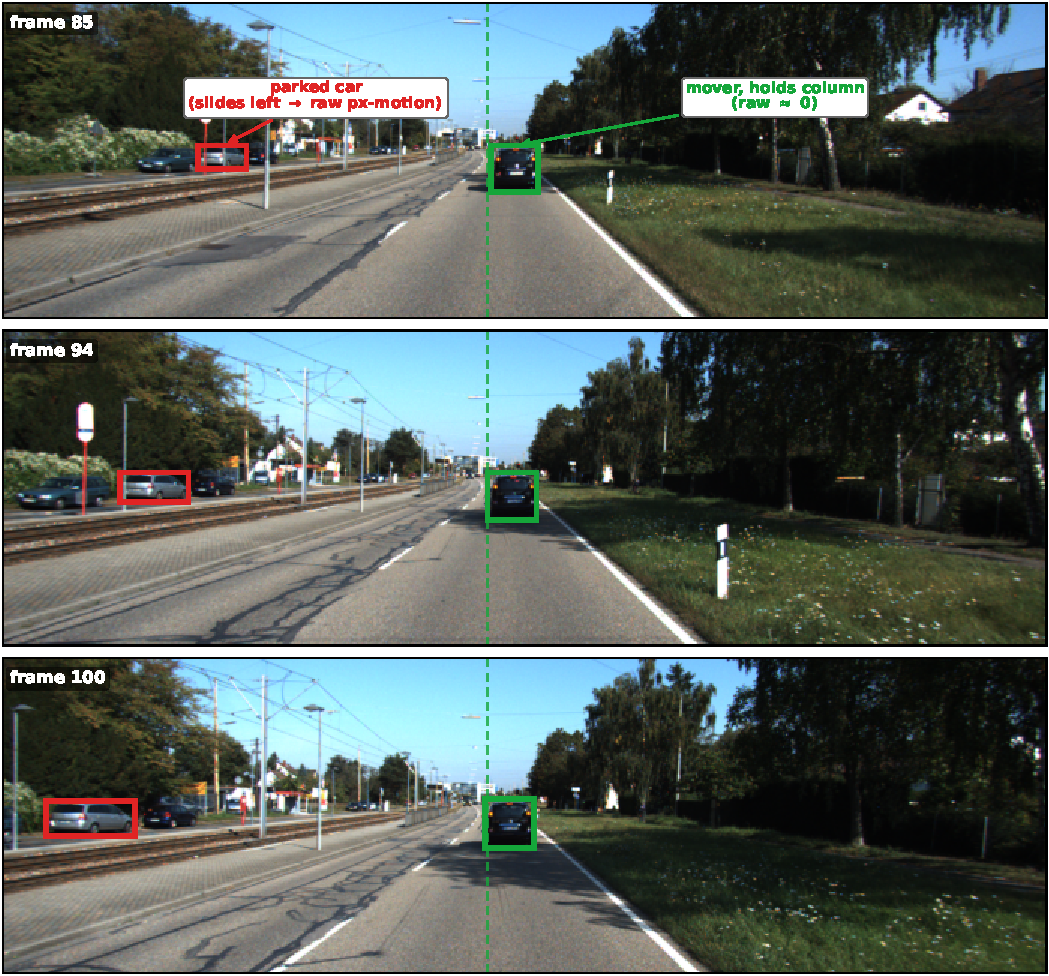
\includegraphics[width=\linewidth]{figures/qualitative.pdf}
\caption{\textbf{Real recovery under camera ego-motion} on ``moving cars'' (Refer-KITTI seq 0005, frames 85/94/100 of a forward-driving clip; the green car moves, the red car is parked). The dashed line marks the mover's image column. \textbf{Red:} the parked car's centroid slides left as the camera passes it (center-$x$ $261\!\to\!104$\,px), so the camera-naive host scores it ``moving'' (false positive), yet its ego-compensated residual is near zero and the module restores it to static. \textbf{Green:} the moving car holds its column (center-$x$ ${\approx}605$, ${<}1$\,px/frame), so the host misses it (false negative), but its nonzero residual --- unlike the static background --- recovers it as moving. Both errors flip from the same host logit through the additive correction.}
\label{fig:qual}
\end{figure}

Figure~\ref{fig:qual} makes the failure mode concrete. The parked car has large raw image displacement because the camera passes it, while the genuinely moving car maintains nearly the same image column. Raw image-plane motion therefore gives the wrong semantic cue in both directions; ego-compensated residual motion restores the distinction. The module runs at $68$ FPS (median $14.8$\,ms/frame excluding host inference), dominated by CPU ORB homography ($14.55$\,ms); the aligner is under $0.2$\,ms.\footnote{An orthogonal appearance re-ranker reaches $45.612$ pooled HOTA on iKUN ($n{=}3$); we do not claim it here.}

\section{Conclusion and Limitations}
\label{sec:conclusion}
A decision-level motion-language module is a targeted correction: it recovers the motion-class referring expressions that camera-naive hosts miss, without touching the appearance majority. The bulk of the recovery comes from aligning a motion descriptor with language at all; ego-compensation is the component that turns the descriptor into a disambiguator, significantly protecting both the moving and the static class. The result suggests that motion-language grounding in moving-camera video should reason over ego-stable trajectories, not raw image-plane displacement. The module keeps the tracker and detector fixed, retrains no host weights, and adds only host-specific scalar calibration. On iKUN~\cite{ikun} it matches published pooled HOTA while lifting the hidden motion class; on FlexHook~\cite{flexhook} V2 it improves pooled HOTA outright.

The limits are bounded. A single ORB/RANSAC homography~\cite{botsort} is approximate under non-planar scenes and strong parallax; our evidence is therefore confined to planar-dominated Refer-KITTI driving footage, with no claim of transfer to handheld, aerial, or strongly non-planar video. A related failure mode is keypoint starvation: a large mover filling the frame leaves little background texture, triggering the identity fallback exactly when compensation is most needed; the snr feature down-weights such frames but does not recover them. Calibration is host-specific and benchmark-level coefficients are not universal hyperparameters. We study two host architectures across three host--split settings, with FlexHook V1/V2 not independent architectural confirmations. Hosts with native temporal memory, such as TempRMOT~\cite{temprmot}, remain out of scope on tested evidence: cascaded trials regressed pooled HOTA rather than improving it.

The broader implication is that camera compensation can serve not only tracking association, but also language grounding. Richer ego-stable trajectory descriptors are the natural next step for camera-naive RMOT hosts.

\bibliographystyle{ACM-Reference-Format}
\bibliography{refs}

\end{document}
